\chapter{Технологический раздел}
\label{cha:impl}

В данном разделе описываются средства, используемые для разработки программного реализации построенного метода, требования для функционирования ПО, описываются результаты тестирования программного продукта.

\section{Выбор средств разработки}

\subsection{Выбор языка программирования}

Для программной реализации описанного метода был выбран язык программирования Python, так как он обладает следующими свойствами:

\begin{itemize}
	\item большая база библиотек для работы с искусственными нейронными сетями, изображениями и математических расчетов;
	\item сочетание функционального, структурного и объектно-ориентированного подходов позволяет кратко описывать необходимые для решения поставленной задачи математические структуры;
	\item кроссплатформенность.
\end{itemize}

Описанные особенности позволяют при помощи Python одинаково удобно реализовывать как научно-исследовательские прототипы, так и коммерческие реализации программного продукта.

\subsection{Выбор среды программирования и отладки}

В качестве среды разработки для языка Python была выбрана кроссплатформенная IDE PyCharm, выбор которой обусловлен следующими предоставляемыми возможностями, упрощающими разработку приложения и способствующими повышению качества исходного кода:

\begin{itemize}
	\item рефакторинг;
	\item навигация по проекту и исходному коду;
	\item встроенный отладчик;
	\item поддержка систем контроля версий;
	\item статический анализ кода.
\end{itemize}

\subsection{Используемые библиотеки}

В процессе реализации были использованы следующие библиотеки:

\begin{itemize}
	\item OpenCV\cite{opencv} -- библиотека для обработки изображений. Использовалась для считывания, записи и реализации предобработки входных данных.
	\item scikit-learn\cite{scikit} -- библиотека для машинного обучения. Используется для форматирования входных данных.
	\item NumPy\cite{numpy} -- библиотека реализаций вычислительных алгоритмов, оптимизированных для работы с многомерными массивами. Используется для упрощения реализации математических операций.
	\item Tensorflow\cite{tf} -- библиотека для машинного обучения. Используется для построения и обучения классификатора.
	\item Keras\cite{keras} -- библиотека машинного обучения. Используется для построения модели классификатора, работающий на базе Tensorflow.
	\item Tkinter -- графическая библиотека. Используется для создания пользовательского интерфейса на базе средств Tk.
\end{itemize}

\section{Система контроля версий}

В процессе разработки программы использовалась система контроля версий Git, позволяющая вносить в проект атомарные изменения, направленные на решения каких-либо задач. В случае обнаружения ошибок или изменения требований, внесенные изменения можно отменить. Кроме того, с помощью системы контроля версий решается вопрос резервного копирования.

Особенности Git:

\begin{itemize}
	\item данная система контроля версий является децентрализованной, что позволяет иметь несколько независимых резервных копий проекта;
	\item поддерживается хостингом репозиториев GitHub;
	\item поддерживается средой разработки PyCharm;
	\item предоставляет широкие возможности для управления изменениями проекта и просмотра истории изменений.
\end{itemize}

\section{Требования к вычислительной системе}

Для запуска программы необходимо иметь установленный на ЭВМ интерпретатор для Python 3.6 с установленными библиотеками. 

Так как выбранный язык программирования является кроссплатформенным, то требований к использованию операционной системы нет.

Обрабатываемые изображения не требуют большого объема оперативной памяти, но классификатор работает с большим числом параметров, поэтому рекомендуемый размер ОЗУ составляет не менее 256 Мб, желательна архитектура x64 (x86-64).

\section{Формат данных}

В качестве входных данных используются RGB изображения в следующих форматах:

\begin{itemize}
	\item BMP -- разработка компании Microsoft. В данном формате хранятся только однослойные растры. Значения пикселей могут иметь разрядности 1, 2, 4, 8, 16, 24, 32, 48 и 64 бит. При 8 и меньше бит в пикселе хранится индекс цвета в таблице цветов, а при большей -- непосредственное значение в цветовой модели RGB.
	\item JPEG -- формат хранения растровых изображений, способный сжимать изображения как с потерями, так и без потерь качества. 
	\item PNG -- графический формат, отличительной способностью которого является возможность хранения значений альфа-канала, отвечающую за прозрачность пикселя.
\end{itemize}

\section{Проектирование архитектуры программного комплекса}

Разрабатываемый программный комплекс состоит из следующих частей:

\begin{itemize}
	\item модуль получения изображения жеста;
	\item модуль предобработки входных данных;
	\item модуль классификации жеста.
\end{itemize}

Формальная модель системы изображена на рисунке \ref{impl:idef0}.

\begin{figure}[!h]
	\centering
	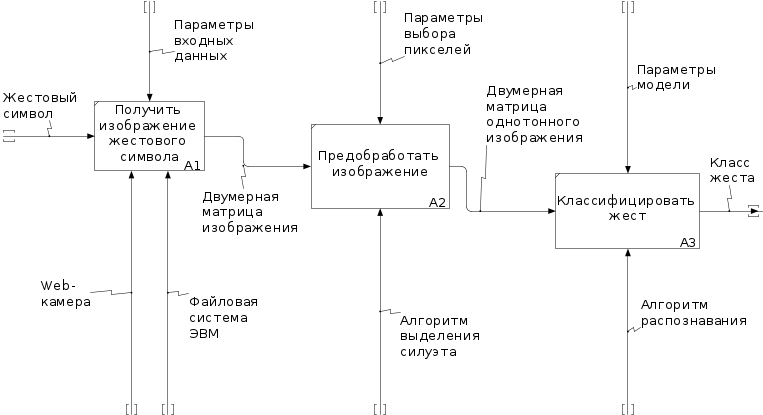
\includegraphics[width=\textwidth]{inc/img/idef0}
	\caption{Формальная модель системы классификации жестовых символов}
	\label{impl:idef0}
\end{figure}

Функционал обучения системы и распознавания жестов разделен на две отдельные подсистемы, объединенных единым хранилищем моделей, из-за разного подхода обработки данных. Итоговая архитектура программного комплекса представлена на рисунке \ref{impl:arch}.

\begin{figure}[!h]
	\centering
	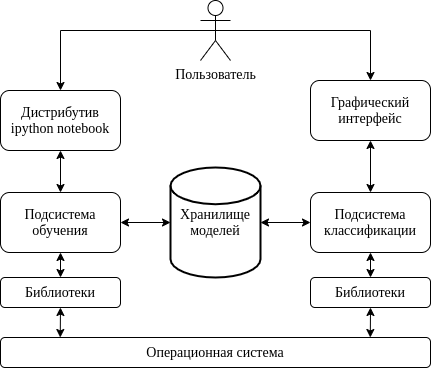
\includegraphics[width=0.55\textwidth]{inc/img/arch}
	\caption{Архитектура программного комплекса}
	\label{impl:arch}
\end{figure}

Основной задачей системы обучения является подготовка моделей классификатора для определенного набора жестовых символов. Для исследования эффективности этапа предобработки входных данных, подсистема обучения способна создавать модели для изображений с предобработкой и без. Функциональные возможности подсистемы обучения представлены на рисунке \ref{impl:train_func}.

\begin{figure}[!h]
	\centering
	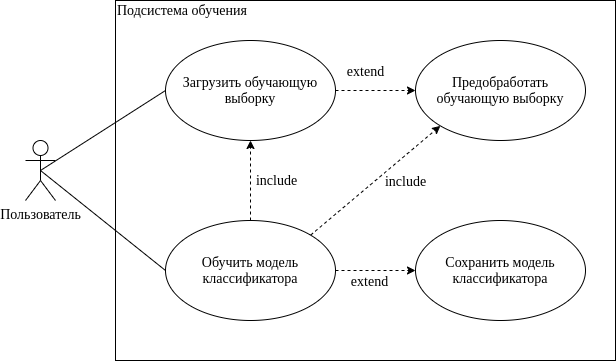
\includegraphics[width=0.6\textwidth]{inc/img/train_func}
	\caption{Функциональные возможности подсистемы обучения}
	\label{impl:train_func}
\end{figure}

Подсистема распознавания жестовых символов выполняет получение изображения с жесткого диска или с Web-камеры, предобработку данных и классификацию жеста. Функциональные возможности подсистемы распознавания жестовых символов изображены на рисунке \ref{impl:run_func}.

\begin{figure}[!h]
	\centering
	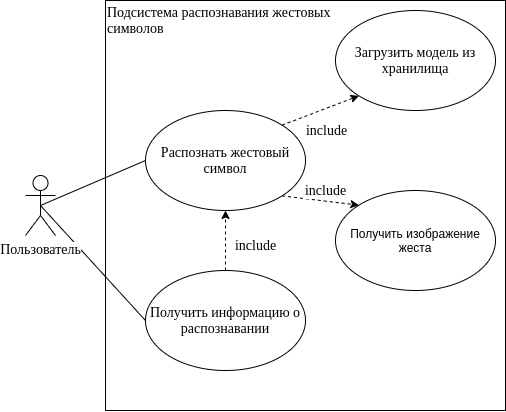
\includegraphics[width=0.6\textwidth]{inc/img/run_test}
	\caption{Функциональные возможности подсистемы распознавания жестовых символов}
	\label{impl:run_func}
\end{figure}

Каждый этап функционирования системы был реализован в виде обособленных модулей с унифицированными API и форматами данных. Функционал данного программного продукта может быть расширен путем добавления новых подсистем, а так же адаптирован под иные источники и форматы изображений жестовых символов.

\section{Построение нейронной сети}

На вход нейронной сети подается черно-белое изображение, полученное на этапе предобработки. Исходный код программной реализации выделения контура кисти руки представлен на алгоритме \ref{app:detector}.

В представлении Tensorflow нейронная сеть является графом потока данных, в котором данные в виде многомерного массива переходят в разные узлы, в процессе чего происходят все необходимые вычисления. Из-за данного подхода процесс описания нейронных сетей с использованием нативного Tensorflow затруднителен. Для упрощения построения моделей можно использовать библиотеку Keras, которая предоставляет простой и удобный способ создания моделей глубокого обучения. Данная библиотека имеет большую базу широко используемых типов слоев искусственных нейронных сетей, а так же предоставляет возможность описывать собственные слои через наследование базового класса Layer.

Алгоритм \ref{imp:init-model} описывает построение КНС. Для преобразования входного изображения в тенсор используется слой layers.Input.

Капсулы первого капсульного слоя, как описано выше, представляют собой комбинацию нескольких сверточных слоев. В следствии этого, реализация данного слоя возможна стандартными слоями библиотеки Keras, как показано на алгоритме \ref{imp:prim}.

Второй капсульный слой нельзя реализовать стандартными средствами пакета layers библиотеки Keras из-за необходимости самостоятельного описания алгоритма динамической маршрутизации. Для этого был описан класс, CapluleLayer, наследованный от класса layers.Layer. Реализация динамической маршрутизации представлена в алгоритме \ref{imp:digit}. Исходный код реализации вычисления формулы \ref{eq:caps-sum} и вычисление длин выходных векторов представлены на алгоритмах \ref{app:squash} и \ref{app:length} соответственно.

Итоговый граф изображен на рисунке \ref{impl:graph}.

\begin{figure}[!h]
	\centering
	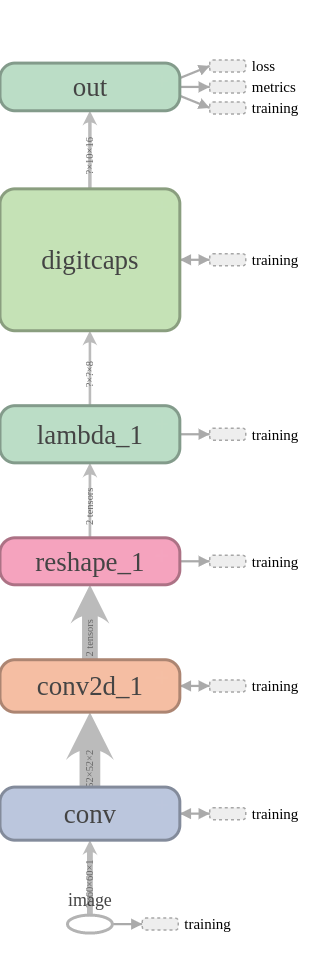
\includegraphics[width=0.3\textwidth]{inc/img/graph}
	\caption{Граф модели}
	\label{impl:graph}
\end{figure}

\section{Руководство пользователя}

\subsection*{Установка программного обеспечения}

Для запуска разработанного программного комплекса требуется установленный на ПК интерпретатор для Python 3. Все необходимые библиотеки указаны в файле requirements.txt, находящемся в корневом каталоге проекта. Средствами каталога программного обеспечения PyPI (Python Package Index) все зависимости устанавливаются выполнением одной команды в терминале:

\textbf{\$ pip3 install -r requirements.txt}

\subsection*{Подсистема обучения}

Обучение классификаторов происходит с помощи Jupyter Notebook -- интерактивной оболочки для языка Python. Данная технология позволяет объединяет код и вывод в окне одного документа, содержащего текст, математические уравнения и визуализации. Такой пошаговый подход обеспечивает быстрый, последовательный процесс разработки, поскольку вывод для каждого блока показывается сразу же.

Для работы и выполнения кода ноутбуков необходимо запустить сервер Jupiter, выполнив в корневом каталоге команду:

\textbf{\$ jupiter notebook}

После этого в стандартном браузере системы откроется сайт с URL http://localhost:8888/tree с файловым менеджером, открытым в корневом каталоге. Для запуска ноутбуков обучения нужно открыть в этом же окне любой файл из папки notebooks и нажать кнопку Run All. Результаты обучения сохраняются в папку data/название выборки/tensorboard.

\subsection*{Подсистема распознавания жестовых символов}

В подсистеме распознавания жестовых символов используется уже обученная нейронная сеть, файл с весовыми коэффициентами которой находится в папке data/название выборки/tensorboard. Для удобства пользователя программное обеспечение поставляется с набором уже обученных классификаторов. Для запуска программы используется команда 

\textbf{\$ python3 main.py}

После запуска программы появляется главное окно (рисунок \ref{impl:main_start}).

\begin{figure}[!h]
	\centering
	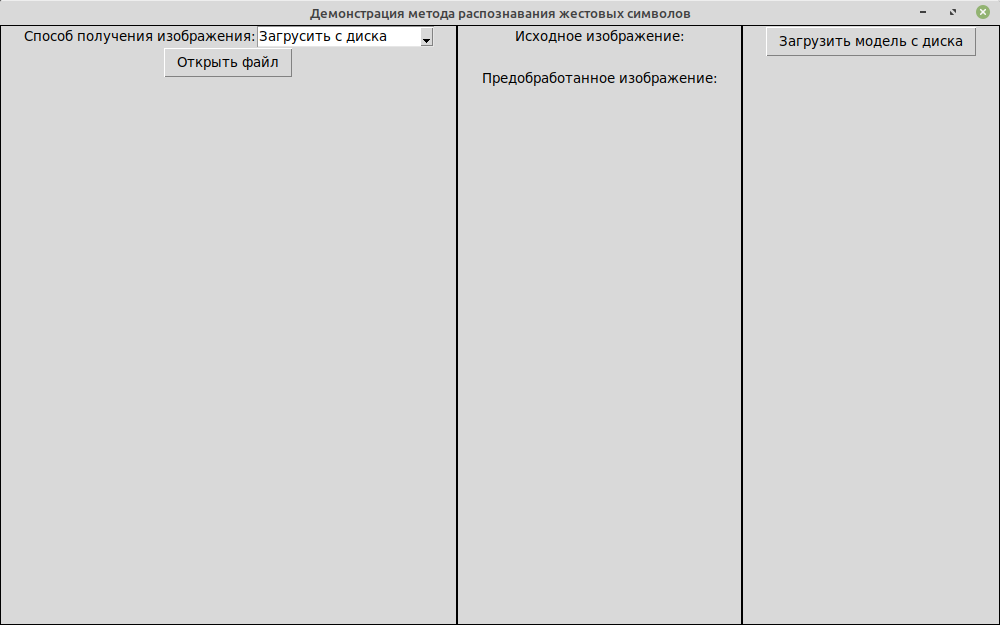
\includegraphics[width=0.7\textwidth]{inc/img/main_start}
	\caption{Окно программы после запуска}
	\label{impl:main_start}
\end{figure}

Визуально область окна разделена на 3 зоны:
\begin{itemize}
	\item Зона загрузки данных. Управляет методом получения изображения. Изначально указан метод <<Загрузить с диска>>, отображающий кнопку <<Открыть файл>>, при нажатии которого открывается диалоговое окно выбора файла изображения. При переключении на метод <<Снять с web-камеры>> открывается окно с демонстрацией видео-потока с web-камеры и кнопкой <<Сделать снимок>> (рисунок \ref{impl:main_webcam}).
	
	\begin{figure}[!h]
		\centering
		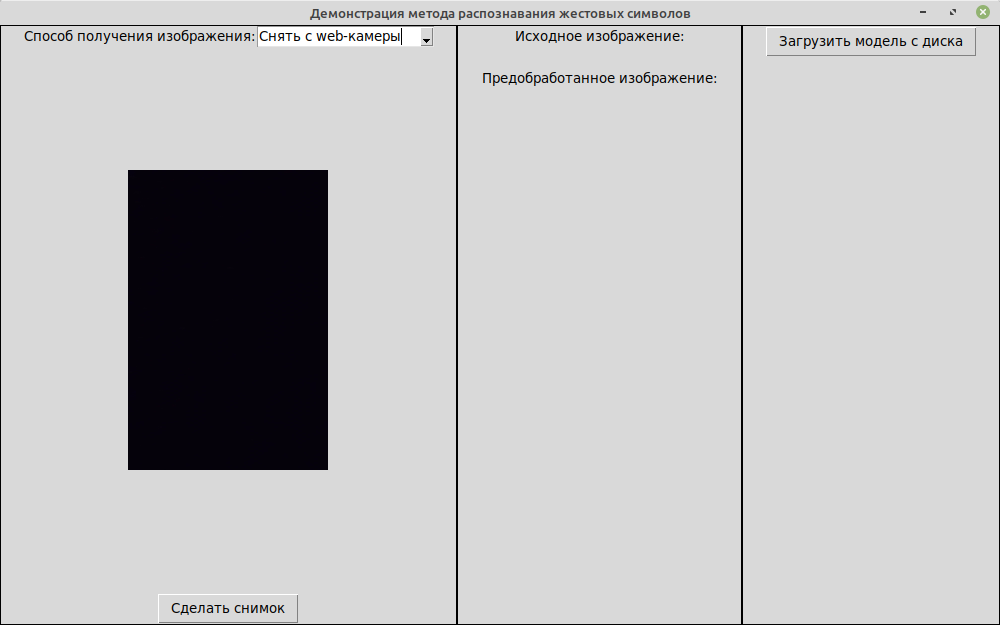
\includegraphics[width=0.7\textwidth]{inc/img/main_webcam}
		\caption{Окно программы в режиме получения изображения с web-камеры}
		\label{impl:main_webcam}
	\end{figure}

	\item Зона предварительно обработки. После получения входных данных отображает два изображения: оригинальное и результат предобработки (рисунок \ref{impl:main}).
	
	\begin{figure}[!h]
		\centering
		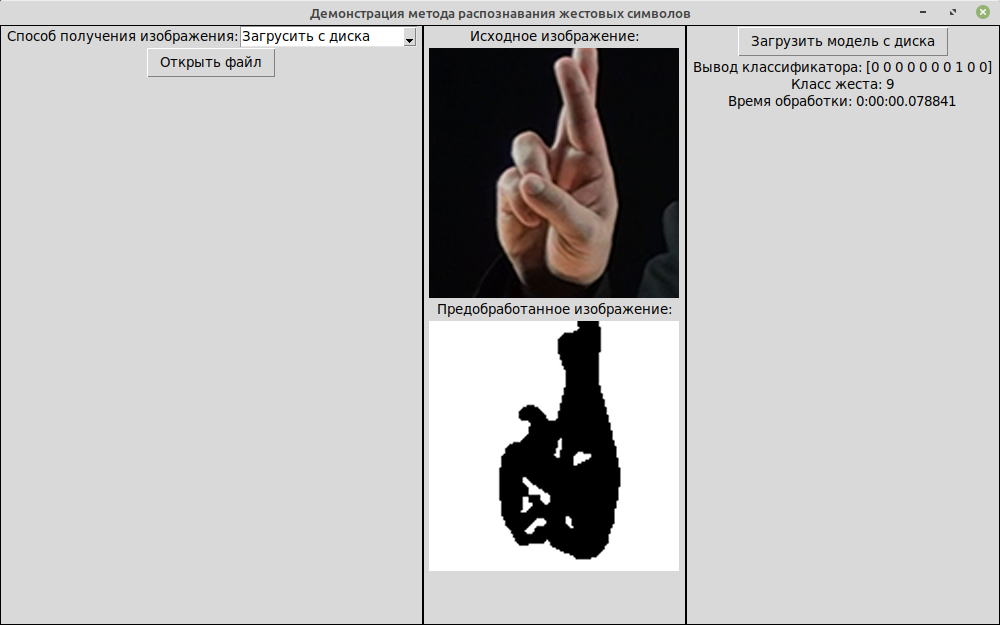
\includegraphics[width=0.6\textwidth]{inc/img/main}
		\caption{Окно программы после классификации}
		\label{impl:main}
	\end{figure}

	\item Зона классификации. Кнопка <<Загрузить модель с диска>> открывает диалоговое окно выбора файла весовых коэффициентов КНС. Ниже отображаются результаты классификации: исходный вывод модели, интерпретированный результат классификации и время полной обработки изображения.
\end{itemize}

\section{Вывод}

Была разработана архитектура программного комплекса для демонстрации работы метода классификации жестовых символов. Процесс обучения и эксплуатации системы выделены в отдельные подсистемы для упрощения разработки. Проведена декомпозиция подсистем на модули, позволяющие расширять функционал программного продукта путем добавления новых модулей.

На основе спроектированной архитектуры был разработан программный комплекс на языке Python с использованием библиотек OpenCV, scikit-learn, NumPy, Tensorflow, Keras и Tkinter.

Продукт был разработан на ЭВМ со следующими характеристиками:

\begin{itemize}
	\item Процессор: Intel© Core™ i5-8250U.
	\item Тактовая частота: 1.60ГГц $\times$ 4
	\item Объем оперативной памяти: 8 Гб.
	\item Графическая карта: Intel Corporation UHD Graphics 620.
	\item Операционная система: Linux Mint 19.3 Cinnamon.
	\item Версия ядра Linux: 5.3.0-53-generic.
\end{itemize}